%% En enkel mall för att skapa en labb-raport.
\documentclass[a4paper, 11pt]{article}
\usepackage[utf8]{inputenc}
\usepackage[swedish]{babel}
\usepackage{amsmath}
\usepackage{amssymb}
\usepackage{listings}
\usepackage[colorlinks=true]{hyperref}
\usepackage[parfill]{parskip}
\usepackage{color}
\usepackage{syntax}
\usepackage{newfloat}
\usepackage{microtype}
\usepackage{amsmath}
\usepackage{graphicx}
\usepackage{mathtools}

\graphicspath{ {./images/} }

\definecolor{codebg}{rgb}{.9,.9,.9}

\DeclareFloatingEnvironment[
  fileext   = logr,
  listname  = {Lista över Grammatik},
  name      = Grammatik,
 % placement = htp
]{Grammar}

\lstset{
	language=erlang,
	basicstyle=\footnotesize\ttfamily,
	numbers=left,
	breaklines=true,
	frame=r,
	captionpos=b,
	showstringspaces=false,
	escapeinside={@*}{*@},
	backgroundcolor=\color{codebg}
}

\hyphenpenalty=900
\hyphenation{prestanda-vinster antingen ut-formad funk-tion-en grunden inter-pretator uppgiftsdeklarationen}

\title{Mandelbrot}
\author{Emil Tullstedt \href{mailto:emiltu@kth.se}{$<$emiltu@kth.se$>$}}
\date{2015-02-19}

\begin{document}

\maketitle

\section{Uppgiften}
\label{sec:uppgiften}
Uppgiften går ut på att implementera en specifikation av Mandelbrotmängden i Erlang. Mandelbrotmängden är en matematisk formell baserad på komplexa tal och utifrån denna generera de effektfulla bilderna som uppstår av att grafiskt synliggöra Mandelbrotmängden.

\section{Ansats}

\subsection{\texttt{cmplx}-modulen}
Modulen \texttt{cmplx} ansvarar för beräkningar med komplexa tal och har fyra funktioner som skapar en representation för, adderar, kvadrerar samt beräknar absolutvärdet på komplexa tal. Ett komplext tal $C = R + I$ representeras i \texttt{cmplx}-modulen som \lstinline${cmplx, Real, Imaginary}$ där \texttt{Real} motsvarar den reella delen $R \in \mathbb{R}$ av det komplexa talet och \texttt{Imaginary} motsvarar den imaginära delen $I \in \mathbb{I}$.

Adderingen av två komplexa tal sker genom att ta det reella värdet $R$ från de bägge talen och addera dem och sedan det imaginära värdet $I$ från bägge talen och addera dem enligt ekvation \ref{equ:addcmplx}.

\begin{equation}\label{equ:addcmplx}
C' = R_1 + R_2 + I_1 + I_2
\end{equation}

För att kvadera ett komplext tal blir det hela lite mer komplicerat, den reella delen blir $R' = R^2 - I^2$ och den imaginära delen blir $I' = 2\times R\times I$. Det nya talet $C^2$ beräknas i ekvation \ref{equ:sqrcmplx}

\begin{equation} \label{equ:sqrcmplx}
C^2 = R^2 - I^2 + 2\times R\times I
\end{equation}

Slutligen implementeras absolutvärdet $|C|\in \mathbb{R}^+$ av $C$. Absolutvärdet extraheras med hjälp av formeln i ekvation \ref{equ:abscmplx}.
\begin{equation} \label{equ:abscmplx}
|C| = \sqrt{R^2+I^2}^+
\end{equation}

Addition, kvadrering och absolutvärde är alla operationer på komplexa tal som behövs för Mandelbrotmängden.

\subsection{\texttt{brot}-modulen}
Modulen \texttt{brot} innehåller två viktiga funktioner, \texttt{test} som undersöker om ett värde ingår i mandelbrotmängden och \texttt{checkN} som används för beräkningen tillhörande \texttt{test}.

\texttt{checkN} är en hjälpfunktion till \texttt{test} som returnerar ett värde $0 \leq n < m$ beroende på om ett komplext tal $C$ ingår i Mandelbrotmängden. \texttt{test} är tillsammans med hjälpfunktionen \texttt{checkN} rekursiv funktion som beskrivs i ekvation \ref{equ:checkn} där värdet $I_n$ är det värdet som returneras när man kallar på \texttt{test} med ett värde $C$ och en maxmängd $m$.

\begin{subequations}\label{equ:checkn}
\begin{align}
Z_{0} &= 0\\
Z_{n} &= Z_{n-1} + C\\
I_n &= \begin{dcases}
	0 & \text{för } |Z_n| < 2 \texttt{ och } n \geq m\\
	I_{n+1} & \text{för } |Z_n| < 2\\
	n & \text{för } |Z_n| > 2\\
\end{dcases}
\end{align}
\end{subequations}

\subsection{\texttt{mandel}-modulen}

\texttt{mandel} sköter tillsammans med \texttt{color} och \texttt{ppm}\footnote{\texttt{color} omvandlar tal till färgvärden och \texttt{ppm} en lista av listor till en bild, ingen av dessa avhandlas i rapporten} genereringen av en bild utifrån ett givet område i Mandelbrottmängden.

\section{Utvärdering}

\begin{figure}[h!]
  \centering
    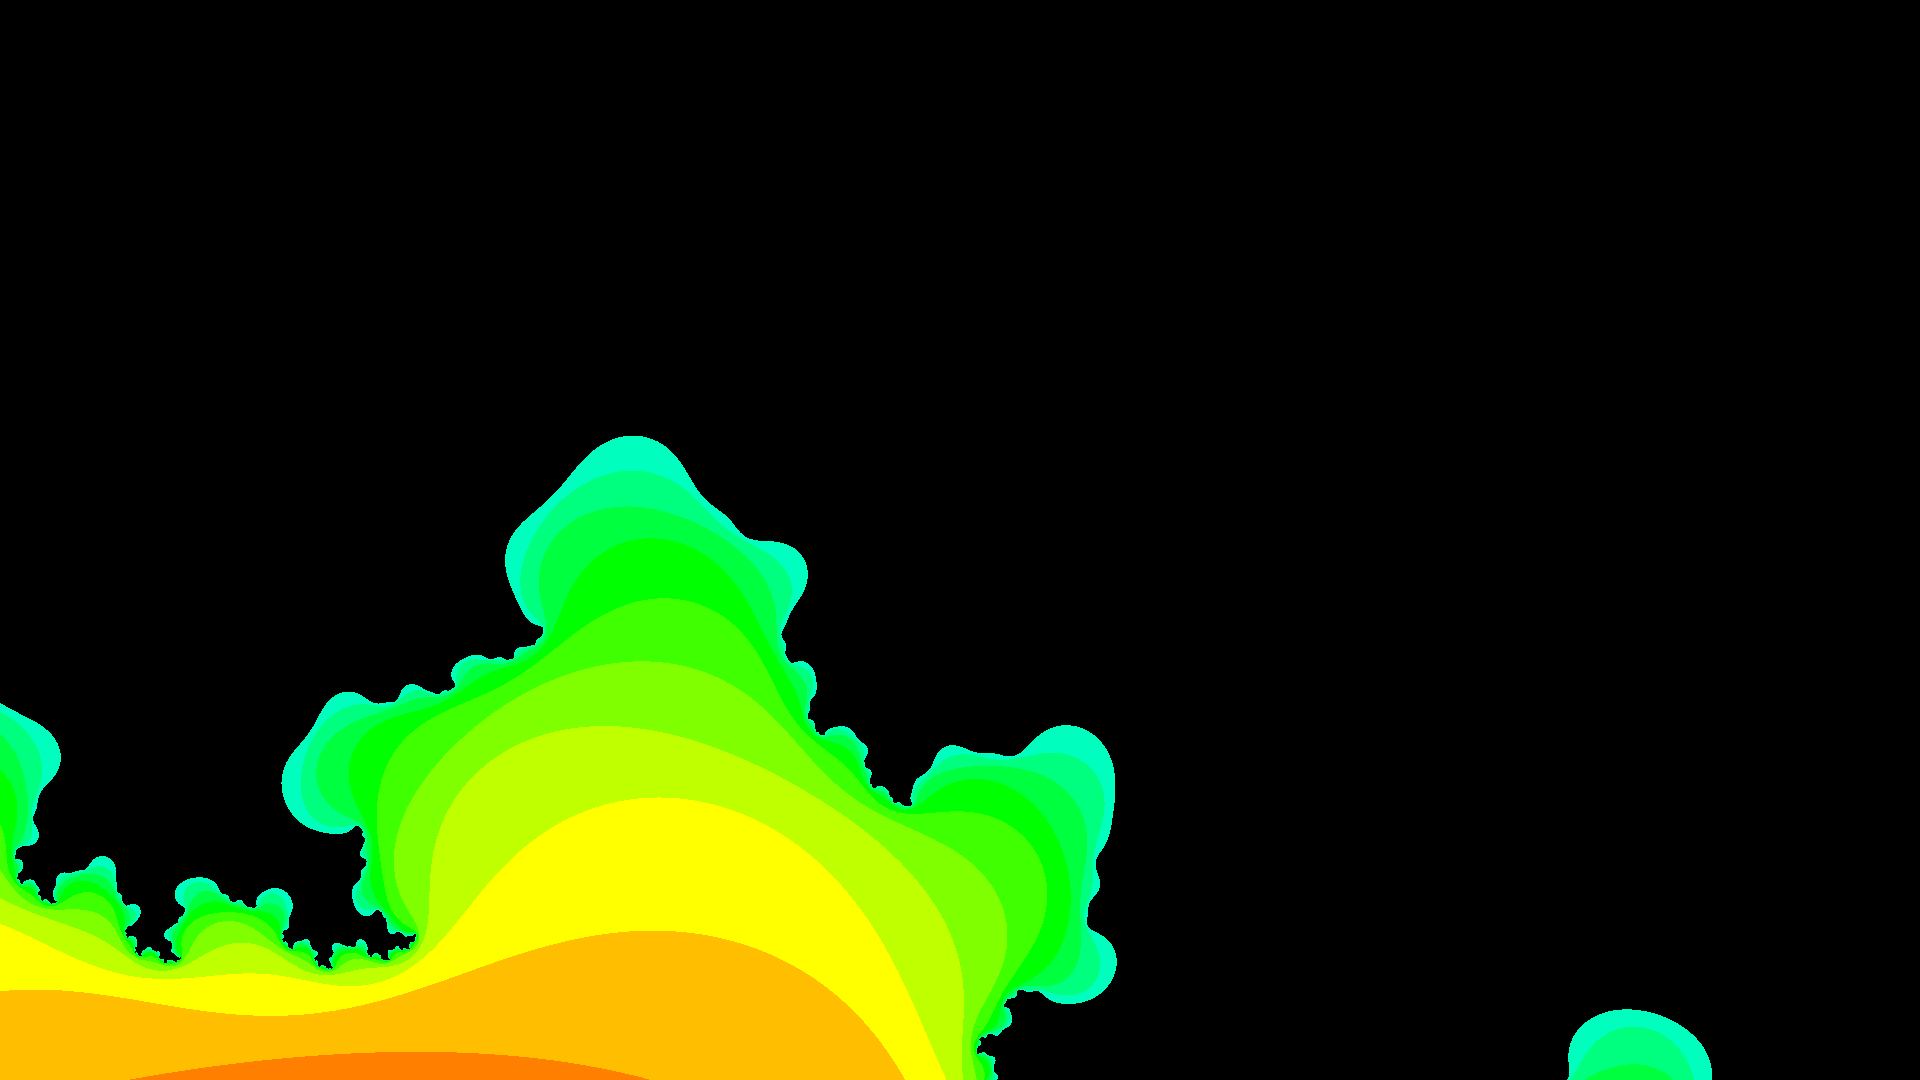
\includegraphics[width=0.7\textwidth]{1080p16zoneb}
  \caption{16 djup \{0.3, 0.5\}, 0.05}
  \label{fig:B16d}
\end{figure}

\begin{table}[h]
\centering
\begin{tabular}{|l|r|r|r|}  
\hline
Tidsåtgång & Upplösning & Djup & Område \{X$_{min}$, X$_{max}$\}, Y\\
\hline
$\sim35$m & 1920x1080p & 4096 --- $2^{12}$ & \{0.25, 0.253\}, 0.001\\
\hline
$\sim70$s & 1920x1080p & 128 --- $2^7$ & \{0.25, 0.253\}, 0.001\\
\hline
$\sim38$s & 1920x1080p & 64 --- $2^6$ & \{0.25, 0.253\}, 0.001\\
\hline
$\sim6$s & 1920x1080p & 8 --- $2^3$ & \{0.25, 0.253\}, 0.001\\
\hline
$\sim55$s & 1920x1080p & 128 --- $2^7$ & \{0.3, 0.5\}, 0.05\\
\hline
$\sim23$s & 1280x720p & 128 --- $2^7$ & \{0.3, 0.5\}, 0.05\\
\hline
$\sim29$s & 1920x1080p & 64 --- $2^6$ & \{0.3, 0.5\}, 0.05\\
\hline
$\sim13$s & 1280x720p & 64 --- $2^6$ & \{0.3, 0.5\}, 0.05\\
\hline
$\sim17$s & 1920x1080p & 32 --- $2^5$ & \{0.3, 0.5\}, 0.05\\
\hline
$\sim7$s & 1280x720p & 32 --- $2^5$ & \{0.3, 0.5\}, 0.05\\
\hline
$\sim10$s & 1920x1080p & 16 --- $2^4$ & \{0.3, 0.5\}, 0.05\\
\hline
$\sim4$s & 1280x720p & 16 --- $2^4$ & \{0.3, 0.5\}, 0.05\\
\hline
\end{tabular}
\caption{Lista över tidsåtgång för generering av olika fraktaler}
\label{tab:timer}
\end{table}

\begin{figure}[h!]
  \centering
    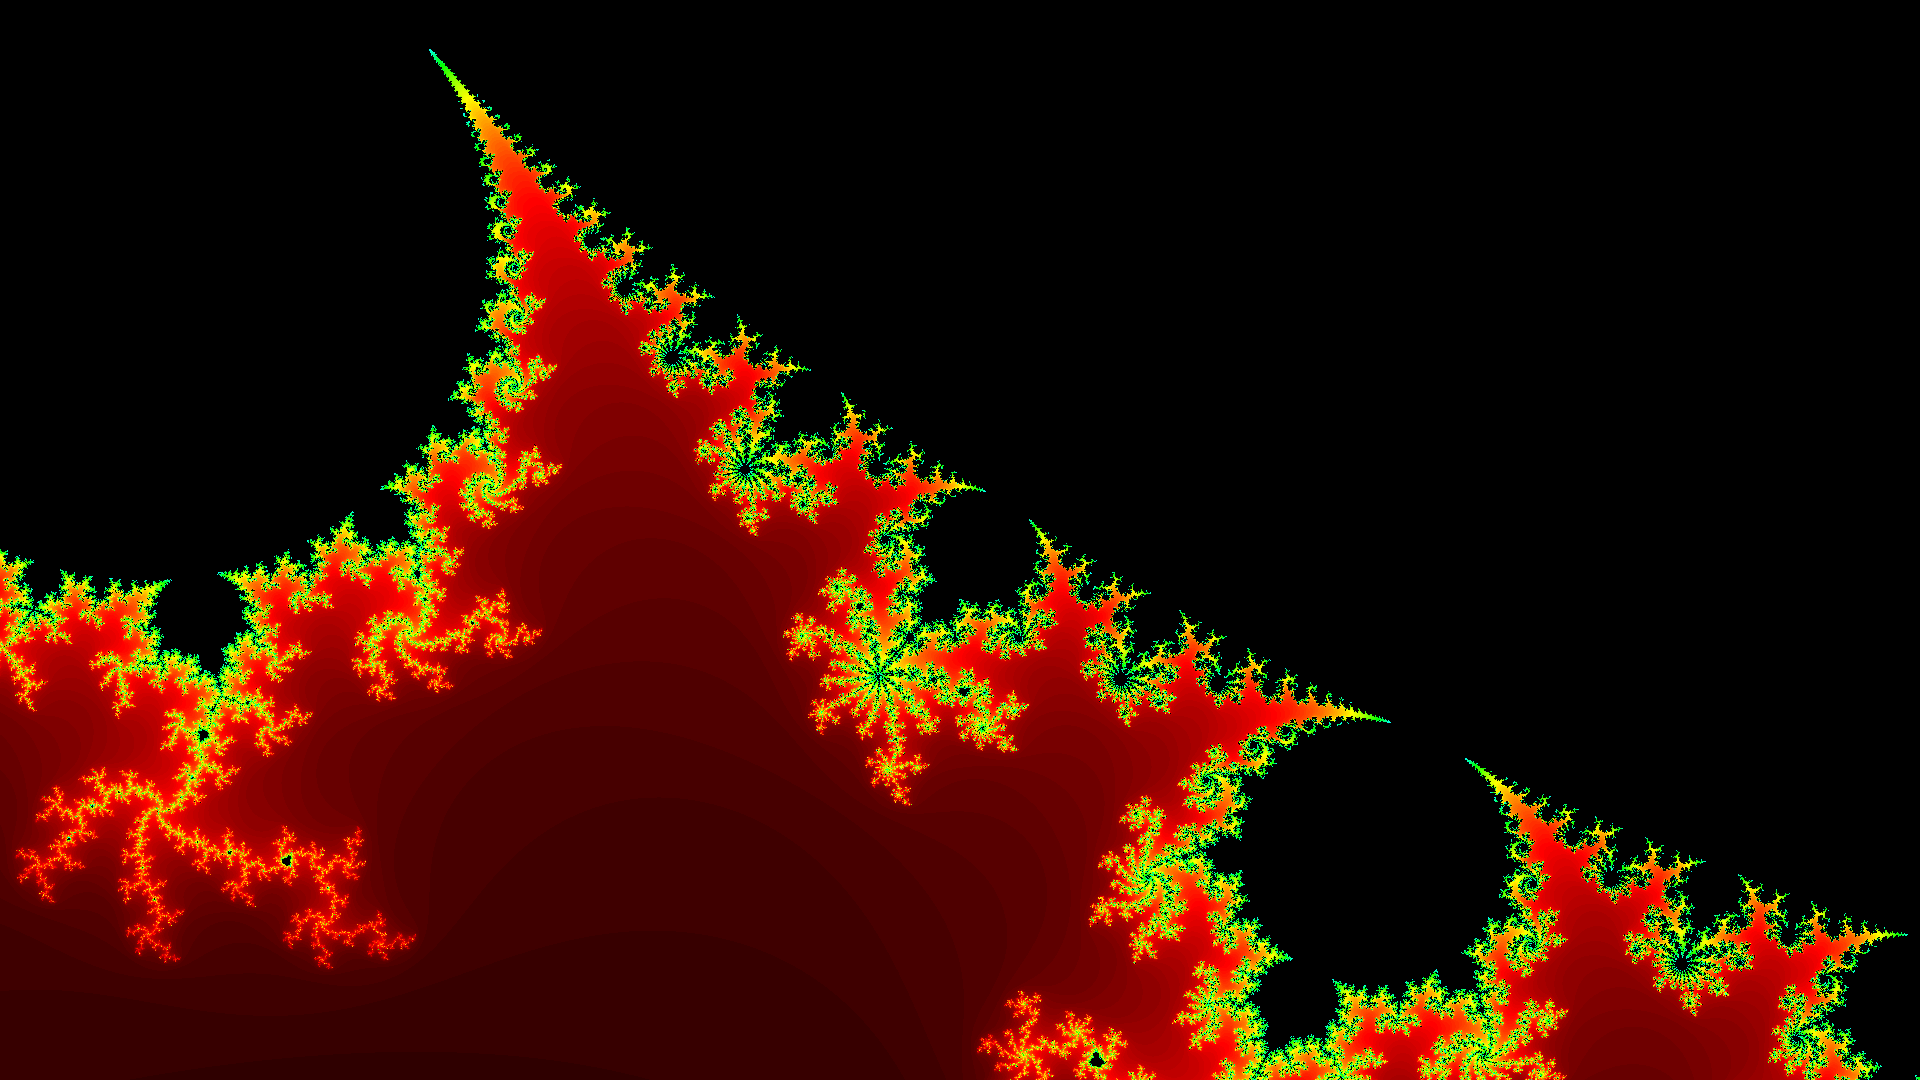
\includegraphics[width=0.7\textwidth]{1080p128zoneb}
  \caption{128 djup \{0.3, 0.5\}, 0.05}
  \label{fig:B128d}
\end{figure}

\begin{figure}[h!]
  \centering
    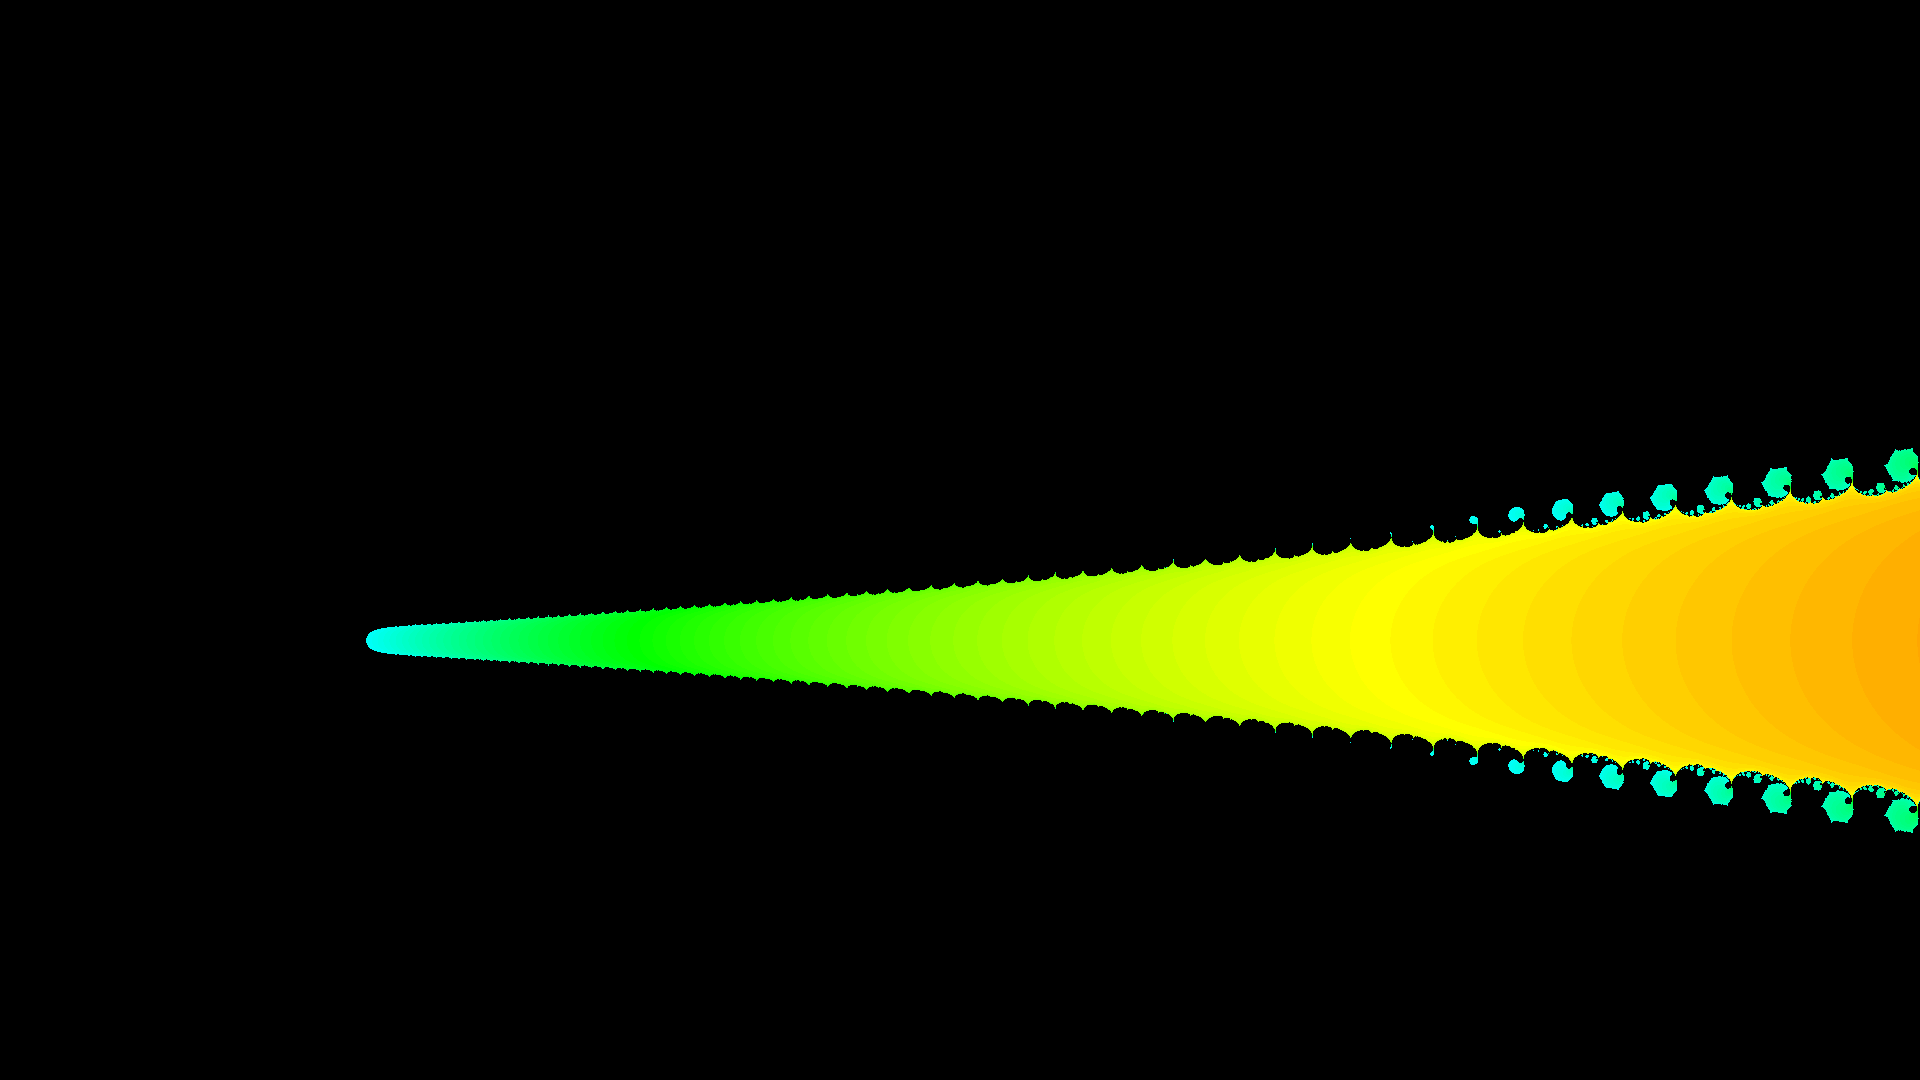
\includegraphics[width=0.7\textwidth]{1080p128zonea}
  \caption{128 djup \{0.25, 0.253\}, 0.001}
  \label{fig:A128d}
\end{figure}

En analys av informationen från tabell \ref{tab:timer} tyder på att djupet och upplösningen har en likvärdig betydelse för tidsåtgången. En dryg halvering av ytan\footnote{1280x720 är $\sim$44\% av 1920x1080} leder till en halvering av tidsåtgången och det syns även att en minskning av djupet leder till motsvarande prestandaförbättringar.

Olika områdens prestanda beror på faktorer där t.ex. bildpunkter som är närmre ytan går snabbare att beräkna än bildpunkter som når botten. Det här är anledningen till att det går $\sim$27\% snabbare att generera bilden i figur \ref{fig:B128d} än bilden i figur \ref{fig:A128d} som är placerad vid ett djupare område i Mandelbrottmängden.

En intressant observation är att området i figur \ref{fig:B16d} och \ref{fig:B128d} är detsamma, och att de uppenbara skillnaderna mellan de figurerna beror helt på djupet. I de fallen när en åskådare observerar Mandelbrotmängden kan det vara intressant att manipulera djupinställningarna för att undersöka hur ett och samma område förändras baserat på hur djupt åskådaren undersöker området.

\section{Sammanfattning}
Uppgiften kändes på det stora taget inte särskilt utvecklande i förhållande från tidigare uppgifter, särskilt inte när raytracer-uppgiften redan hade avhandlats på ett seminarium. Det var en rolig uppgift, men tidsåtgången för själva uppgiften var minimal.

\end{document}
